\chapter{Introducción específica}

En este capítulo se presenta un resumen de los conceptos más relevantes acerca de la red TCN y su implementación en las formaciones de Trenes Argentinos, y se detallan las diferentes tecnologías utilizadas para el desarrollo del dispositivo de captura.

\section{La red TCN}

La red TCN es una combinación jerárquica de dos buses de datos en los que se transmite información dentro de una formación ferroviaria. El \textit{Multifunction Vehicle Bus} (MVB) interconecta los diferentes dispositivos presentes dentro de cada vehículo, y el \textit{Wire Train Bus} (WTB) interconecta los diferentes vehículos. Los componentes de la red TCN están estandarizados en la norma IEC 61375-1. En la figura~\ref{fig:tcn-mvb-wtb} se muestra un diagrama simplificado de la arquitectura TCN.

\begin{figure}[htbp]
	\centering
    {
        \fontfamily{phv}
        \fontsize{9pt}{9pt}\selectfont
        \input{./Figures/tcn-mvb-wtb.pdf_tex}
    }
	\caption[\textit{Wire Train Bus} y \textit{Multifunction Vehicle Bus}]{\textit{Wire Train Bus} y \textit{Multifunction Vehicle Bus}.\footnotemark}
    \label{fig:tcn-mvb-wtb}
\end{figure}
\footnotetext{Dibujo del tren por Freepik\\(\url{https://www.freepik.com/free-vector/collection-different-types-trains_1114167.htm})}

Dado que el dispositivo desarrollado se conecta al bus MVB, a continuación se exponen las características principales de este bus de comunicación.

\subsection{El bus MVB}

El bus MVB interconecta diferentes dispositivos ubicados en el mismo vehículo o en diferentes vehículos que no son separados con frecuencia. El MVB puede direccionar hasta 4095 dispositivos de distintos tipos, desde simples sensores y actuadores hasta equipos programables.

La estructura de MVB sigue el modelo OSI \cite{ISO7498-1}, que establece siete capas de abstracción en el proceso de transmisión de datos.
En las capas inferiores del protocolo MVB se establecen las características del medio físico y la estructura de las tramas y telegramas.
A continuación, se describen estos conceptos, que son los más relevantes para el desarrollo de este trabajo.

\subsection{Capa física}

El bus MVB ofrece tres opciones de medios físicos para la capa inferior:

\begin{itemize}
\item El medio \textit{Electrical Short Distance} (ESD), para distancias de hasta 20~m, que soporta hasta 32 dispositivos por segmento, con transceptores de tipo RS-485.
\item El medio \textit{Electrical Middle Distance} (EMD), para distancias de hasta 200~m, que soporta hasta  32 dispositivos por segmento, con transformadores y transceptores compatibles con la norma IEC 61158-2 \cite{iec61158_2}.
\item El medio \textit{Optical Glass Fibre} (OGF), para distancias de hasta 2000~m, y soporta conexiones punto a punto o subredes de topología tipo estrella.
\end{itemize}

Puede haber diferentes buses en un vehículo, interconectados mediante un \textit{gateway} al bus WTB.
También es posible que el bus MVB abarque más de un vehículo, y en este caso la norma recomienda el medio EMD.
Un ejemplo de esta configuración se ilustra en la figura~\ref{fig:emd-esd-wtb}.

\begin{figure}[htbp]
	\centering
    {
        \fontfamily{phv}
        \fontsize{9pt}{9pt}\selectfont
        \input{./Figures/medios.pdf_tex}
    }
	\caption[MVB abarcando tres vehículos]{MVB abarcando tres vehículos.}
    \label{fig:emd-esd-wtb}
\end{figure}

En la figura~\ref{fig:segmento} se ilustra un segmento EMD.
Cada dispositivo conectado a un segmento EMD tiene dos conectores D-sub de 9 pines (DE-9) que van, respectivamente, al dispositivo anterior y siguiente en el segmento. Los dispositivos en los extremos del segmento tienen un terminador.

\begin{figure}[htbp]
	\centering
    {
        \fontfamily{phv}
        \fontsize{9pt}{9pt}\selectfont
        \input{./Figures/segmento-emd.pdf_tex}
    }
	\caption[Un segmento EMD]{Un segmento EMD.}
    \label{fig:segmento}
\end{figure}

En la figura~\ref{fig:pines} se muestra la configuración de pines de los conectores.
La transmisión de la señal digital se realiza mediante la tensión diferencial entre los pares Data\_N y Data\_P. La norma permite que haya una única línea (A) o dos líneas (A y B) para proporcionar redundancia.

\begin{figure}[htbp]
	\centering
    {
        \fontfamily{phv}
        \fontsize{8pt}{8pt}\selectfont
        \input{./Figures/db9-emd.pdf_tex}
    }
	\caption[Configuración de pines del conector D-sub de 9 pines del medio EMD]{Configuración de pines del conector DE-9 del medio EMD. Se omite por simplicidad la interconexión de los pines 6 a 9, que se utilizan para los terminadores.}
    \label{fig:pines}
\end{figure}

\subsection{Tramas}
\label{sec:tramas}

Se denomina ``trama'' a un paquete de datos transmitido por un dispositivo.
En el bus MVB se transmiten dos tipos de tramas:

\begin{itemize}
\item La trama \textit{master}, que es transmitida únicamente por el dispositivo maestro del bus.
\item La trama \textit{slave}, que es transmitida por un dispositivo esclavo en respuesta a una trama \textit{master}.
\end{itemize}

Todos los medios MVB operan a una velocidad unificada de 1,5~Mbit/s.
La información se transmite utilizando una codificación Manchester, que combina en una única señal la información y el \textit{clock}.

La transmisión de una trama se compone de un delimitador inicial (SD) de 9 bits de duración, los datos de la trama, una secuencia de verificación (CS) de 8 bits y un delimitador final (ED) de 2 bits de duración.
En los datos de la trama y la secuencia de verificación, un ``1'' se transmite como una transición negativa en el medio de una celda de bit, y un ``0'' se transmite como una transición positiva.
Los delimitadores de inicio para las tramas \textit{master} y \textit{slave} son diferentes, y se denominan MSD y SSD.
En la figura~\ref{fig:manchester} se muestra a modo de ejemplo la transmisión de una trama \textit{master} en el medio EMD.

\begin{figure}[htbp]
	\centering
    {
        \fontfamily{phv}
        \fontsize{8pt}{8pt}\selectfont
        \input{./Figures/manchester.pdf_tex}
    }
	\caption[Transmisión de una trama master]{Transmisión de una trama \textit{master}.}
    \label{fig:manchester}
\end{figure}


\subsection{Telegramas}

Una secuencia de una trama \textit{master} seguida de una trama \textit{slave} conforman un telegrama, como se muestra en la figura~\ref{fig:telegrama}.

\begin{figure}[htbp]
	\centering
    {
        \fontfamily{phv}
        \fontsize{8pt}{8pt}\selectfont
        \input{./Figures/telegrama.pdf_tex}
    }
	\caption[Un telegrama MVB]{Un telegrama MVB.}
    \label{fig:telegrama}
\end{figure}

Las tramas \textit{master} tienen una longitud fija de 16 bits (sin contar los delimitadores), e incluyen:

\begin{itemize}
\item Un código de 4 bits llamado \texttt{F\_code}, que indica el tipo y tamaño de la trama \textit{slave} esperada a continuación.
\item Un campo de 12 bits, que puede contener una dirección de destino, o parámetros específicos al \texttt{F\_code}.
\end{itemize}

Todos los dispositivos conectados al bus decodifican la trama \textit{master}. El dispositivo encuestado luego responde con su trama \textit{slave}, que a su vez puede ser recibida por otros dispositivos.

\subsection{Variables}

Son de particular interés los telegramas con \texttt{F\_code} entre 0 y 4, que se denominan \texttt{Process\_Data}.
En este caso, el campo de 12 bits contiene una dirección lógica que hace referencia a un puerto.
Cada puerto está asociado unívocamente a una variable, que puede contener uno o más valores como la velocidad actual, la tensión de red, el estado de las puertas, etc.
Cada dispositivo \textit{slave} almacena uno o más puertos, y al ser encuestado responde con el valor actual de la variable correspondiente.

\section{Red TCN en las formaciones de Trenes Argentinos}

En la figura~\ref{fig:tms} se muestra un diagrama simplificado de la topología de la red TCN en una sección de 3 vehículos EMU de una formación de Trenes Argentinos. En el diagrama se observa que los buses MVB están implementados con el medio físico EMD.

\begin{figure}[htbp]
	\centering
    {
        \fontfamily{phv}
        \fontsize{8pt}{8pt}\selectfont
        \input{./Figures/tms.pdf_tex}
    }
	\caption[Topología de la red TCN en una formación de Trenes Argentinos]{Topología de la red TCN en una formación de Trenes Argentinos.}
    \label{fig:tms}
\end{figure}

\pagebreak

En la figura~\ref{fig:rcme} se muestra una fotografía de uno de los dispositivos presentes en la cabina del conductor de una formación de la línea Mitre. Se trata del módulo de comunicación RCMe, que controla las puertas, el sistema de aire acondicionado y el sistema de información al pasajero. En el panel frontal del módulo RCMe, los conectores DE-9 X1 y X2 (destacados en la figura) corresponden al bus MVB.

\begin{figure}[htbp]
	\centering
	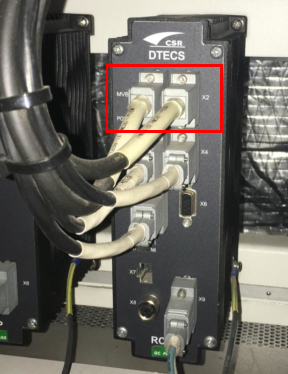
\includegraphics[width=0.5\textwidth]{./Figures/RCMe.pdf}
	\caption[El módulo de comunicación RCMe]{El módulo de comunicación RCMe presente en un EMU. Los dos conectores DE-9 destacados corresponden al bus MVB.}
    \label{fig:rcme}
\end{figure}

La pantalla HMI (\textit{Human Machine Interface}), también ubicada en la cabina del conductor, tiene un modo de operación que permite visualizar el valor de algunas variables que son transmitidas periódicamente en forma de \texttt{Process\_Data}. En la figura~\ref{fig:hmi} se puede observar que en el puerto 0 hay una variable de 16 bits cuyo valor binario actual es 1100 0001 0110 0101, o 33702 si se interpreta como un número decimal.

\begin{figure}[htbp]
	\centering
	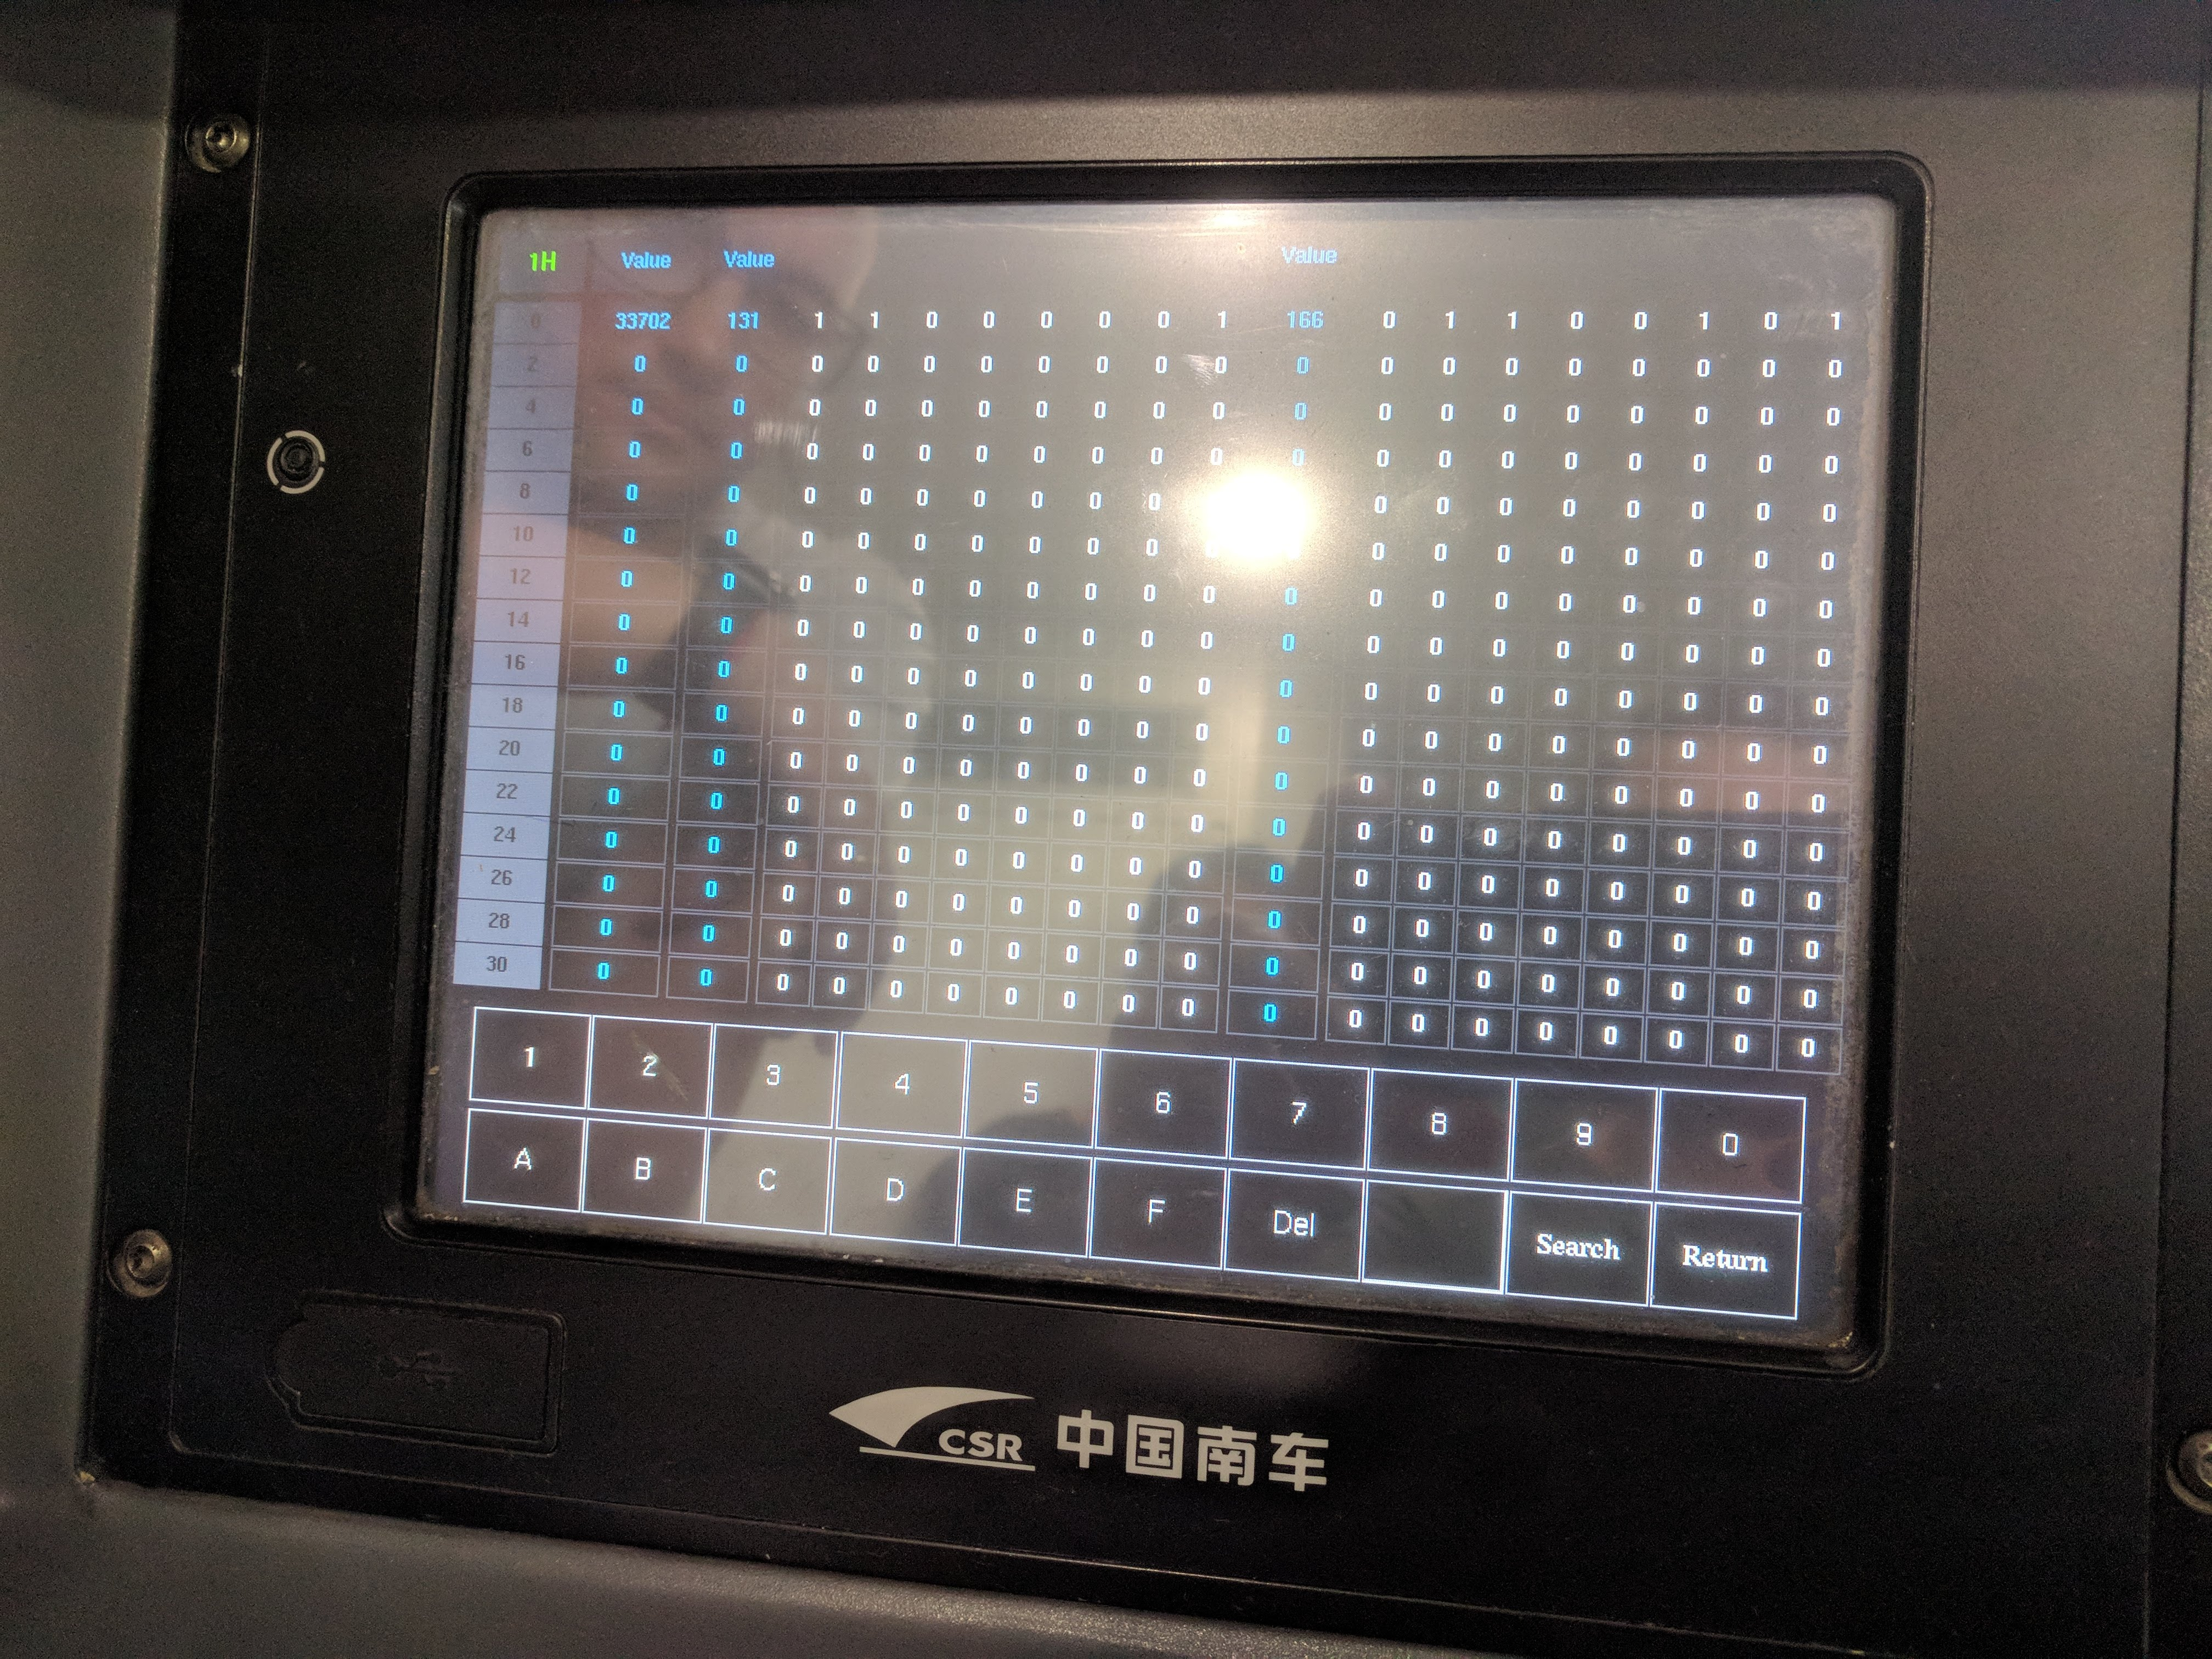
\includegraphics[width=1\textwidth]{./Figures/hmi.jpg}
	\caption[El HMI mostrando algunas variables]{El HMI mostrando algunas variables.}
    \label{fig:hmi}
\end{figure}

\section{Componentes del sistema}

A continuación, se describen las principales tecnologías utilizadas para el desarrollo del dispositivo de captura.

\subsection{EDU-CIAA}

La EDU-CIAA \cite{web:ciaa} es una plataforma de desarrollo de hardware libre basada en el microcontrolador NXP LPC4337 \cite{web:lpc4337} (dual core ARM Cortex-M4F y Cortex-M0), diseñada para la enseñanza de la programación y el desarrollo de sistemas embebidos en Argentina y otros países de habla hispana.
Esta placa cuenta con múltiples interfaces de entrada/salida, como puertos USB, Ethernet, CAN, UART, I²C, SPI, ADC y DAC.

La EDU-CIAA se utilizó para desarrollar un generador de señal MVB que permitió probar el funcionamiento del dispositivo de captura sin necesidad de conectarlo en una formación ferroviaria. El diseño del generador se describe en la sección \ref{sec:generador}.

\subsection{Raspberry Pi}

La Raspberry Pi \cite{web:rpi} es una computadora de placa única (SBC, por sus siglas en inglés) de bajo costo y tamaño reducido, diseñada por la \textit{Raspberry Pi Foundation} para promover la enseñanza de la informática básica en las escuelas y países en desarrollo.
Entre sus capacidades se encuentran el procesamiento de video en alta definición, conectividad inalámbrica y soporte para una gran cantidad de periféricos, lo que la convierte en una opción popular para una amplia gama de proyectos, desde la automatización del hogar hasta la robótica y la creación de servidores web.

El dispositivo de captura desarrollado en este trabajo está basado en la Raspberry Pi. Su diseño se describe en la sección \ref{sec:hardware}.

\subsection{Analizador lógico VKTECH y Sigrok}

El analizador lógico VKTECH \cite{vktech} es un dispositivo que permite capturar y analizar señales digitales en sistemas electrónicos. El dispositivo provee 8 canales que pueden capturar con una frecuencia de muestreo de hasta 24MHz, y cuenta con una interfaz USB 2.0 para conectar a una PC.

Sigrok \cite{sigrok} es un software libre y de código abierto que proporciona una plataforma para la adquisición y análisis de datos de múltiples tipos de instrumentos de medición, incluyendo analizadores lógicos, osciloscopios y multímetros. La herramienta es compatible con una amplia gama de dispositivos y marcas, lo que permite la integración de diferentes equipos y protocolos de comunicación en un solo entorno de software. Además, Sigrok ofrece una interfaz gráfica intuitiva y fácil de usar, así como una API para el desarrollo de aplicaciones personalizadas.

En este trabajo se utilizó el analizador lógico VKTECH y Sigrok en la fase de investigación, para realizar capturas del tráfico del bus MVB y analizarlas, como se menciona en las secciones \ref{sec:capturas} y \ref{sec:decodificacion}.

El dispositivo de captura desarrollado también utiliza el analizador lógico VKTECH y Sigrok para capturar el tráfico del bus en tiempo real, como se describe en las secciones \ref{sec:hardware} y  \ref{sec:software}.

\subsection{Python}

Python \cite{web:python} es un lenguaje de programación interpretado, de alto nivel y de propósito general. Está diseñado para ser fácil de aprender y cuenta con una sintaxis clara y legible.
Además tiene una amplia variedad de librerías y frameworks disponibles que permiten desarrollar aplicaciones en diferentes áreas, como ciencia de datos, inteligencia artificial, automatización y desarrollo web.

En este trabajo se utilizó el lenguaje Python en la fase de investigación, para decodificar las primeras capturas realizadas en la formación, como se describe en la sección \ref{sec:capturas}.

\subsection{Go}

Go \cite{web:go} es un lenguaje de programación de código abierto desarrollado por Google.
Se trata de un lenguaje de alto nivel, compilado, con tipos estáticos y recolector de basura.
Es sintácticamente similar al lenguaje C, pero se caracteriza por su enfoque en la concurrencia, la eficiencia y la simplicidad en la escritura de código.

Se utilizó el lenguaje Go para escribir el software del dispositivo de captura que corre en la Raspberry Pi, como se describe en la sección \ref{sec:software}.
